
%(BEGIN_QUESTION)
% Copyright 2010, Tony R. Kuphaldt, released under the Creative Commons Attribution License (v 1.0)
% This means you may do almost anything with this work of mine, so long as you give me proper credit

A heat exchanger is used to lower the temperature of sulfuric acid (H$_{2}$SO$_{4}$) exiting an exothermic reactor in an acid manufacturing process, using water as the coolant.  An automatic control valve will eventually be installed in the water line, but for now a hand (manual) valve performs the role of coolant throttling over a range of 0 to 25 GPM (gallons per minute):

$$\includegraphics[width=15.5cm]{i00741x01.eps}$$

An experienced instrument technician is summoned to test this heat exchanger system and determine what kind of valve characterization (quick-opening, linear, equal-percent) is best for throttling the water flow.  The technician proceeds to set the manual valve to different positions while recording the three pressure gauge readings and the flow rate (measured by a flowmeter not shown in this illustration).  The results are shown in this table:

% No blank lines allowed between lines of an \halign structure!
% I use comments (%) instead, so that TeX doesn't choke.

$$\vbox{\offinterlineskip
\halign{\strut
\vrule \quad\hfil # \ \hfil & 
\vrule \quad\hfil # \ \hfil & 
\vrule \quad\hfil # \ \hfil & 
\vrule \quad\hfil # \ \hfil \vrule \cr
\noalign{\hrule}
%
% First row
Water flow & Gauge \#1 & Gauge \#2 & Gauge \#3 \cr
%
\noalign{\hrule}
%
% Another row
0 GPM & 48 PSI & 0 PSI & 0 PSI \cr
%
\noalign{\hrule}
%
% Another row
15 GPM & 23 PSI & 2.3 PSI & 0.8 PSI \cr
%
\noalign{\hrule}
%
% Another row
25 GPM & 6 PSI & 5 PSI & 1.5 PSI \cr
%
\noalign{\hrule}
} % End of \halign 
}$$ % End of \vbox

After examining these results, the technician declares ``We'll definitely need equal-percentage trim on this valve.  No way will a linear control valve give us good results.''

\vskip 10pt

Explain the rationale behind the technician's decision.  What is it exactly about the pressure readings that suggest a linear-characteristic valve will not give good results over the flow range of 0 to 25 GPM?  Conversely, what sort of pressure measurements {\it would} suggest a linear-characteristic control valve would suffice?

\underbar{file i00741}
%(END_QUESTION)





%(BEGIN_ANSWER)

Here's a hint: calculate the {\it differential pressure} across the valve for each flow rate, then determine how stable that $\Delta P$ is.

%(END_ANSWER)





%(BEGIN_NOTES)

The $\Delta P$ varies significantly from no flow to full flow, which is {\it the} cause of valve characteristic distortion: namely causing control valves with inherently linear characteristics to behave very non-linearly.  An equal-percentage valve will do much better in this application where the $\Delta P$ varies so wildly across the flow range.

%INDEX% Final Control Elements, valve: characterization

%(END_NOTES)


